\chapter{Extensible Record Stores}
%from age 285 to 313
Extensible record stores are database systems akin to \textbf{Google’s
BigTable system}.
\begin{itemize}
    \item A "Bigtable" is a sparse, distributed, persistent multi-dimensional stored map
    \item It is indexed by \textbf{row key, column key and timestamp}
    \item A \textbf{value} in the map is an uninterpreted array of bytes, also called string
    \item MAP: (row:string, column:string, time:int64) \(\leftarrow\) string
\end{itemize}
These databases have tables as their basic data structure although with a highly flexible column management; they implement the concept of \textbf{column families} that act as containers for subsets of columns.

\section{Logical Data Model}
Extensible record stores do not use the normalization paradigm from RDBMSs. Instead they encourage a certain amount of \textbf{data duplication} for the sake of \textit{better query locality} and more \textit{efficient query execution}.

While the design in the relational model is centered around entities and later on normalization, an extensible record store first of all a typical query workload should be identified and data modeled around this workload accordingly. 

What extensible record stores do to organize these key-value pairs is adding another structural dimension the \textbf{column family}:
\begin{itemize}
    \item It groups columns that are often accessed simultaneously in a typical query
    \item The columns inside are called \textbf{column qualifier}
    \item The full \textbf{column name} consists of the column family name and the column qualifier
    \item \textbf{Value} for each column in a row
    \item \textbf{Row keys} link column of the same entity. However, there is no way of specifying foreign key constraints between different column families and no referential integrity is ensured
\end{itemize}

The \textbf{advantages} of column families are the following:
\begin{itemize}
    \item They provide data locality by storing data inside a column family together on disk
    \item They provide dynamic addition of new columns (at run time)
\end{itemize}
And the following \textbf{characteristics}:
\begin{itemize}
    \item They have to be created before used
    \item Columns families are fixed for a table
    \item There can be infinitely many columns in each column family
\end{itemize}

\begin{figure}[!hbp]
    \centering
    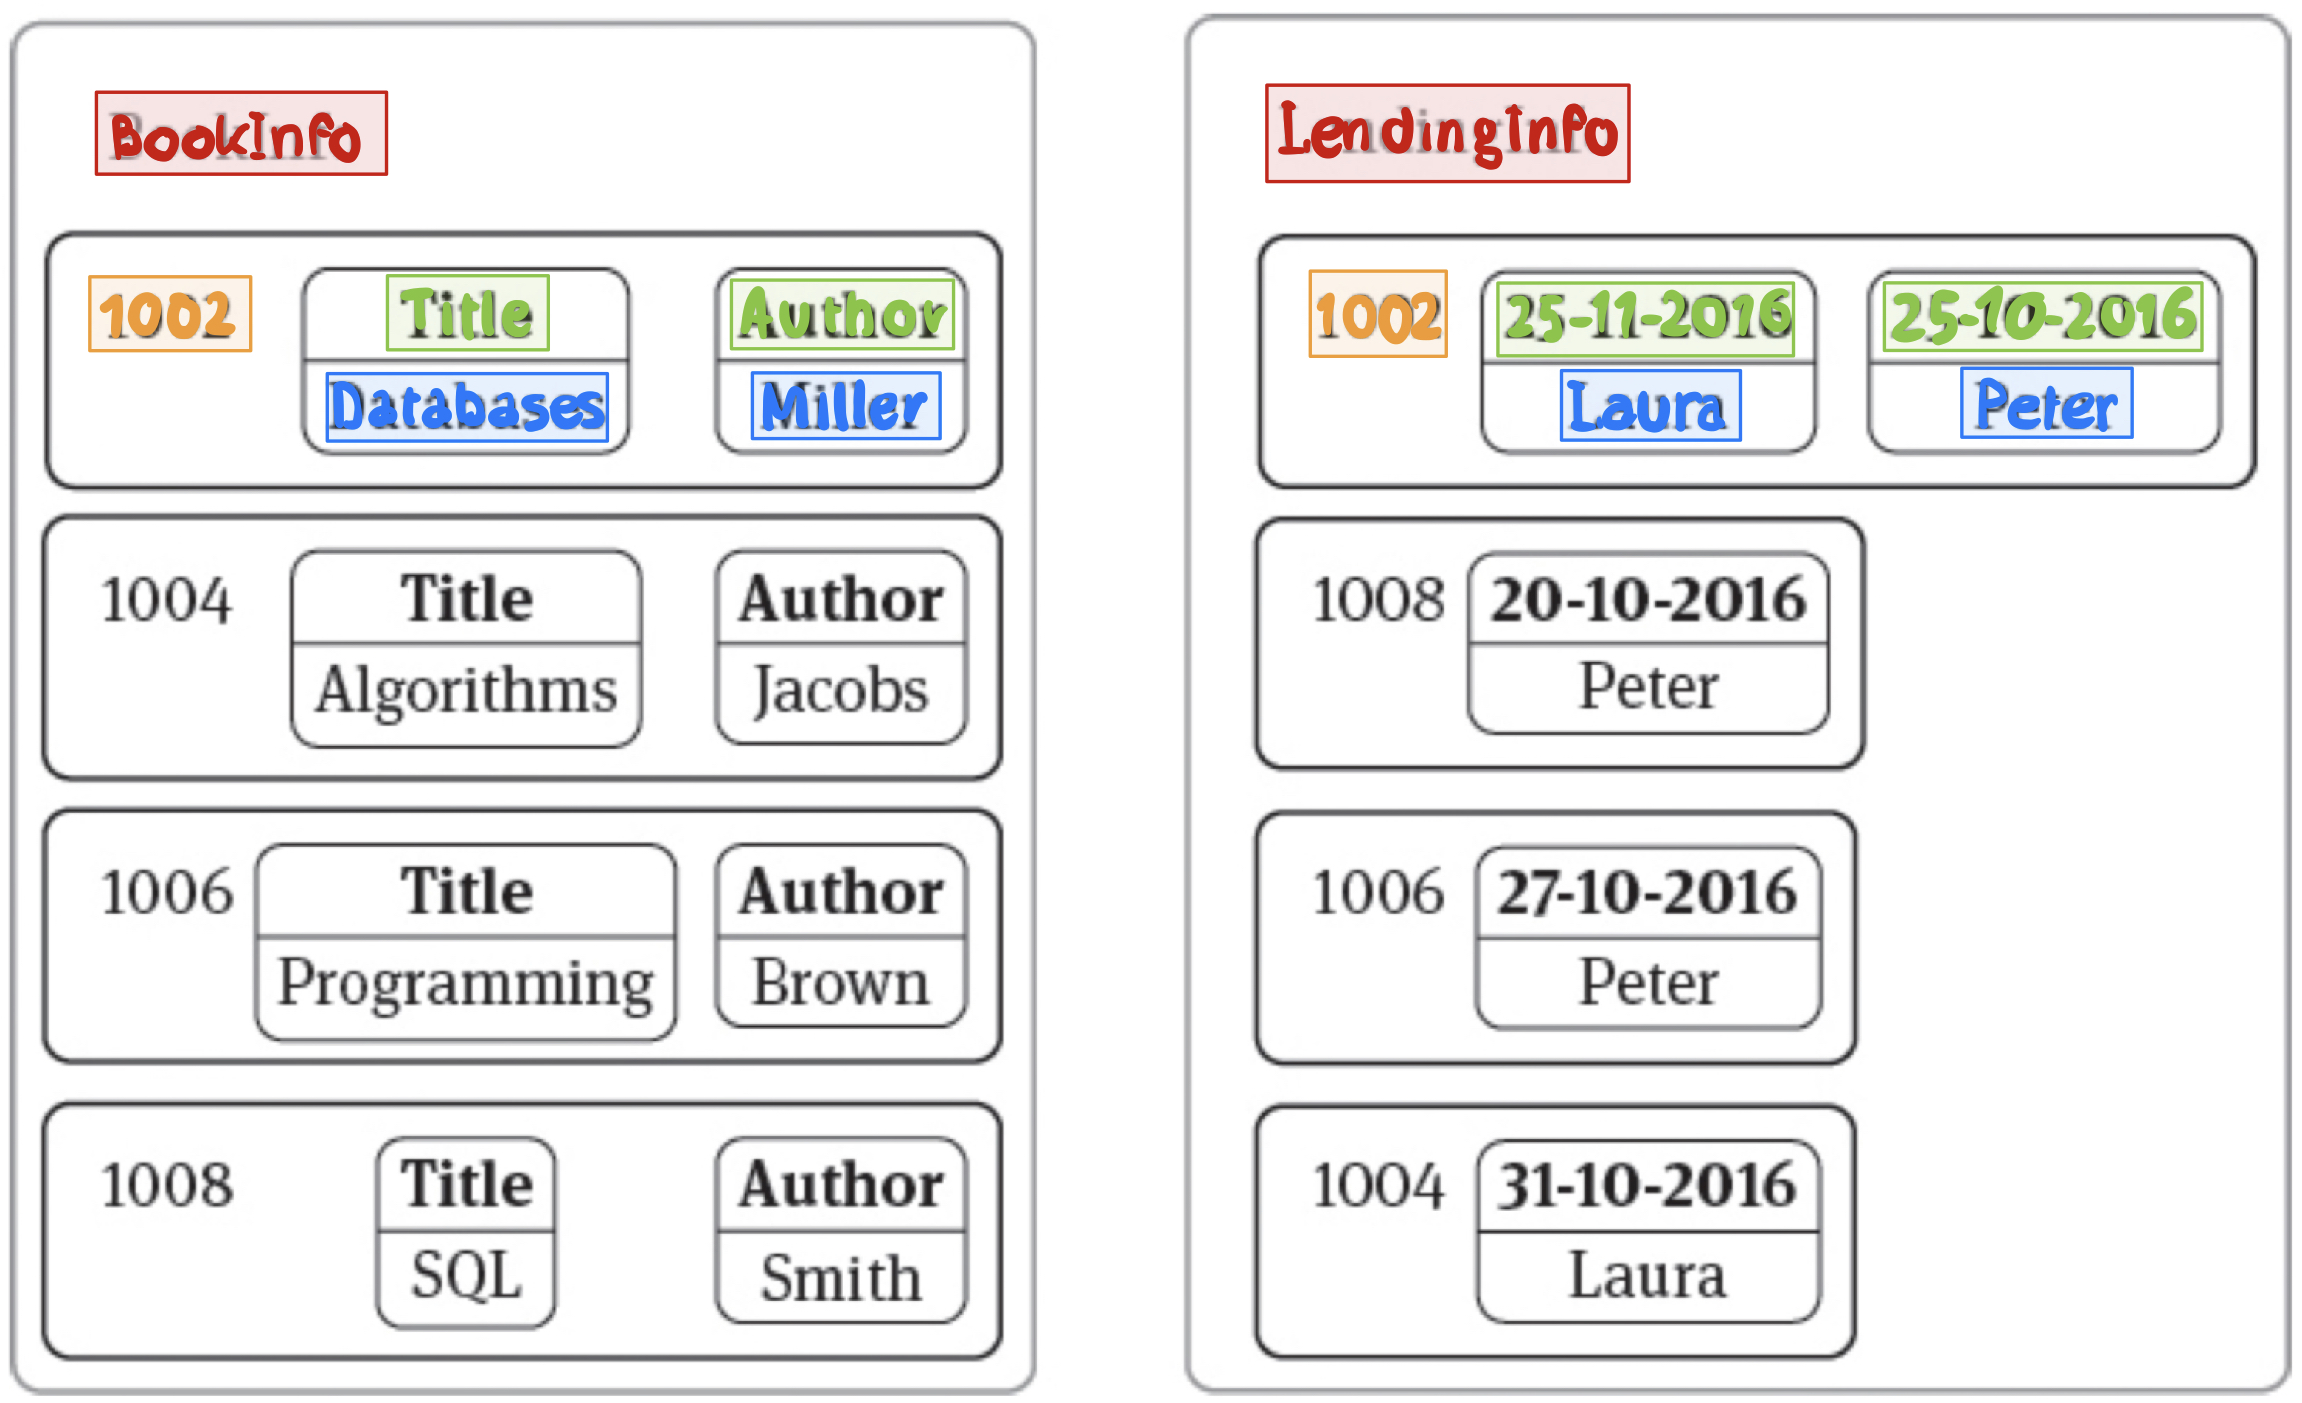
\includegraphics[width=0.90\linewidth]{images/AdvancedDataManagment/extensible_record_store/names_definition.jpeg}
    \caption{\textcolor{red}{Column Families}, \textcolor{green}{Column Qualifiers}, \textcolor{blue}{Values}, \textcolor{orange}{Row Keys}}
\end{figure}

At this point we also see the \textit{flexibility} of how columns can be added to rows, indeed one row can have different columns than other rows inside the same column family. This is why extensible record stores are good at storing \textbf{sparse data:} 
\begin{itemize}
    \item An extensible record store just \textit{ignores} values that are not present and \textit{no null values} are included in rows.
    \item The \textbf{concatenation} of \textit{row key}, \textit{column family name} and \textit{column qualifier} identifies a \textbf{cell} in the extensible record store
    \item The \textbf{full key} in order to access to a specific cell is in the form of:
    \[rowkey:columnfamily:columnqualifier\]
\end{itemize}

Extensible record stores offer the convenient feature of \textbf{ordered storage:}
\begin{itemize}
    \item While the relational data model is set-based and the order of the output basically depends on the DBMS
    \item Extensible record stores sort the data internally
    \begin{itemize}
        \item Inside a \textit{column family}, the rows are sorted by their \textbf{row keys}
        \item Inside a \textit{row} the columns are sorted by their \textbf{qualifiers}
    \end{itemize}
\end{itemize}

Other extensible record stores (like Cassandra) offer data types for row keys and column qualifiers and hence sorting can be done according to the data type and may differ from the binary order.

\begin{figure}[!hbp]
    \centering
    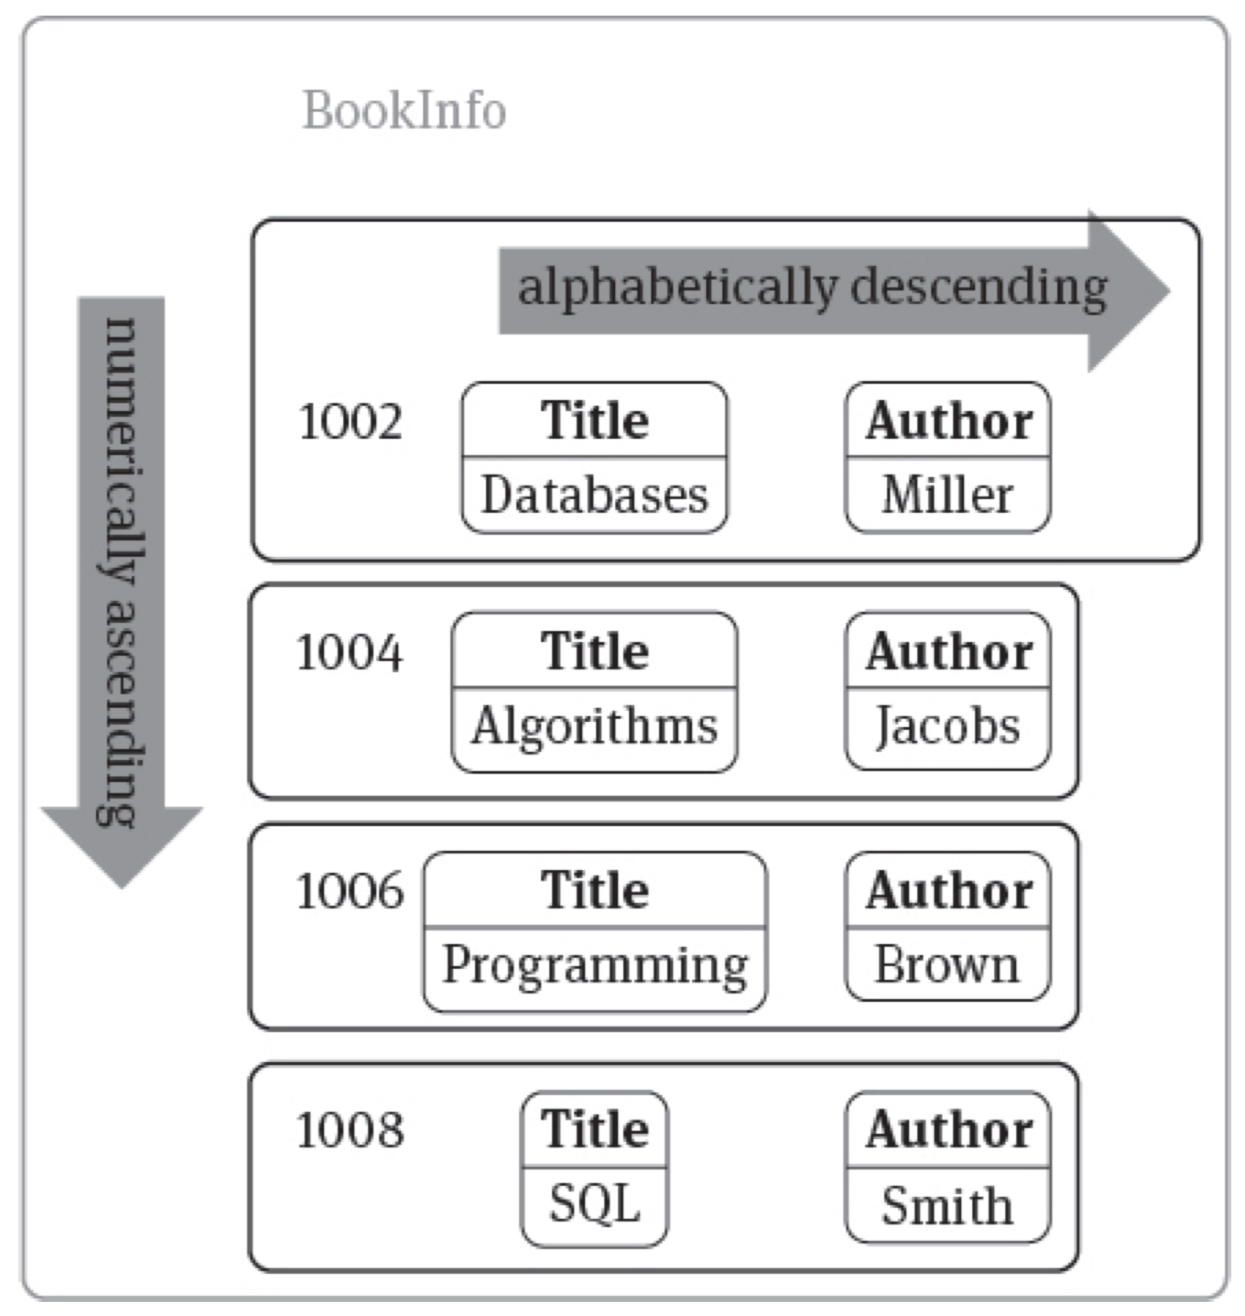
\includegraphics[width=0.50\linewidth]{images/AdvancedDataManagment/extensible_record_store/BookInfo.jpeg}
    \caption{Ordering features of BookInfo}
\end{figure}

\begin{figure}[!hbp]
    \centering
    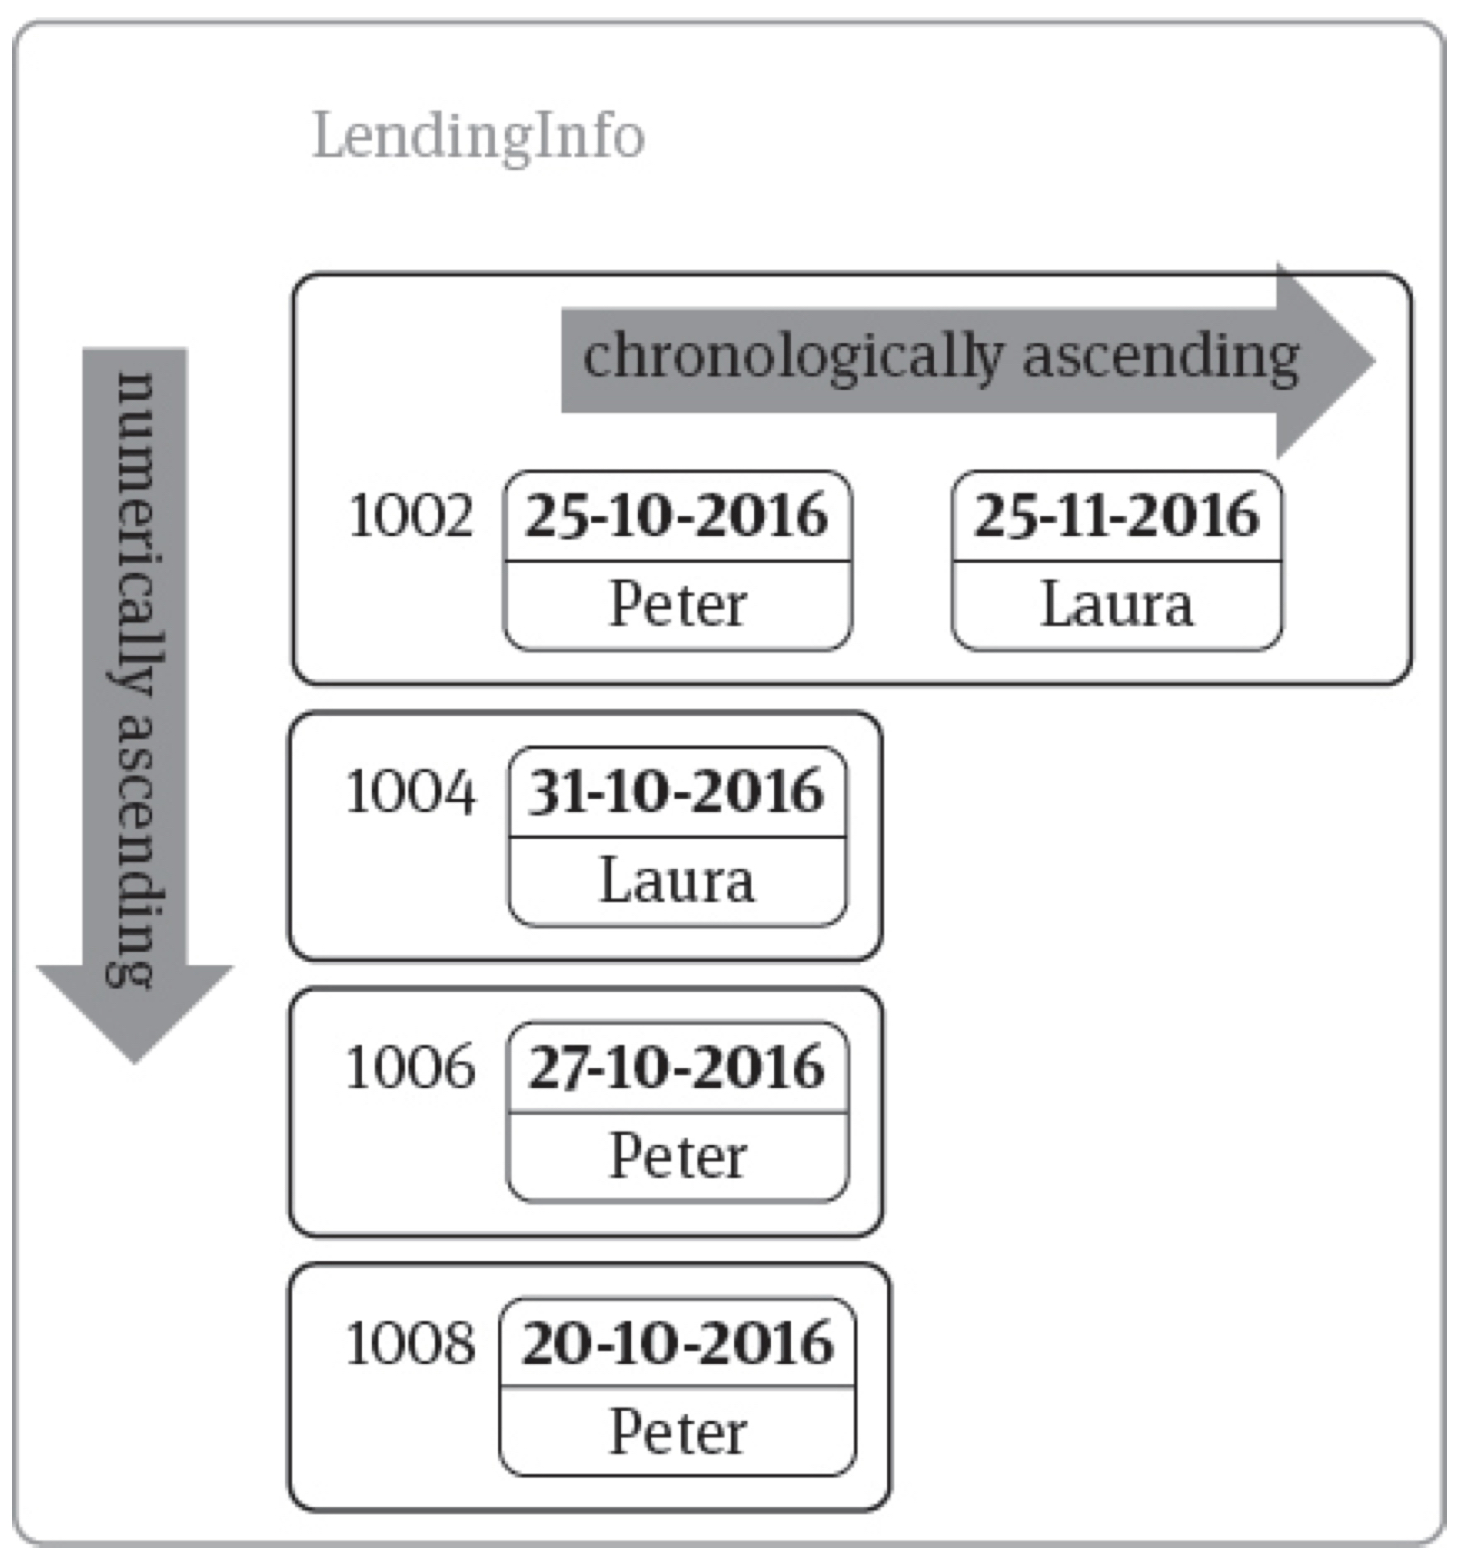
\includegraphics[width=0.50\linewidth]{images/AdvancedDataManagment/extensible_record_store/LendingInfo.jpeg}
    \caption{Ordering features of LendingInfo}
\end{figure}

\newpage
With these ordering features, extensible record stores are particularly well-suited for identifying \textbf{contiguous sequences of columns}.

\vspace{0.5cm}
\centerline{"What are the names of those readers who have to return
books on or before 31-10-2016?"}
\vspace{0.5cm}

To answer this query we have to find out what is following. The columns with column qualifiers less than or equal to 31-10-2016. But \textbf{due to the ordering} the matching columns are stored in a \textit{consecutive range} and that we do not have to search further once we have reached a column qualifier greater than 31-10-2016.

Last but not least, some extensible record stores add \textit{one more dimension} to the row-column family-column space: \textbf{time}.
\begin{itemize}
    \item Each insert or update is accompanied by a \textbf{timestamp} and it can be specified by the user
    \item Extensible record stores provide an \textbf{automatic versioning} of column values
    \item When a read command \textit{without an explicit timestamp} is issued on a cell, the \textit{most recent} version is returned
    \item Versioning can further be configured by specifying a \textit{maximum threshold} for the amount of stored version. 
    \begin{itemize}
        \item The \textbf{oldest version} will \textit{automatically be discarded} once a new version is stored and the maximum value is exceeded
    \end{itemize}
    \item Another option for \textbf{automatic discarding} is to specify a \textbf{time-to-live value} for each cell:
    \begin{itemize}
        \item When the specified time span has \textit{elapsed}, the corresponding \textit{version} of the cell is \textbf{deleted}
    \end{itemize}
\end{itemize}

Furthermore, extensible record stores usually do not make a distinction between inserts and updates. Instead, a
\textbf{put command} is provided that checks whether there is an existing cell for the given key:
\begin{itemize}
    \item If there is, the \textit{value} for the key will be \textbf{updated}
    \item Otherwise a \textit{new cell} is \textbf{inserted}
\end{itemize}
This is why this operation is sometimes called an \textbf{upsert}.

\section{Physical storage}
Extensible record stores use several techniques for \textbf{efficient query answering and recovery.}

\subsection{Memtables and immutable sorted data files}
\subsubsection{Writing to memory tables and data files}
Extensible record stores implement a \textit{write-optimized storage model}
\begin{itemize}
    \item All data records written to the on-disk store will only be appended to the existing records
    \item Once written, these records are read-only and cannot be modified, they are \textbf{immutable}
    \item Any modification must be simulated by appending a new record in the store
\end{itemize}


\begin{figure}[!h]
    \centering
    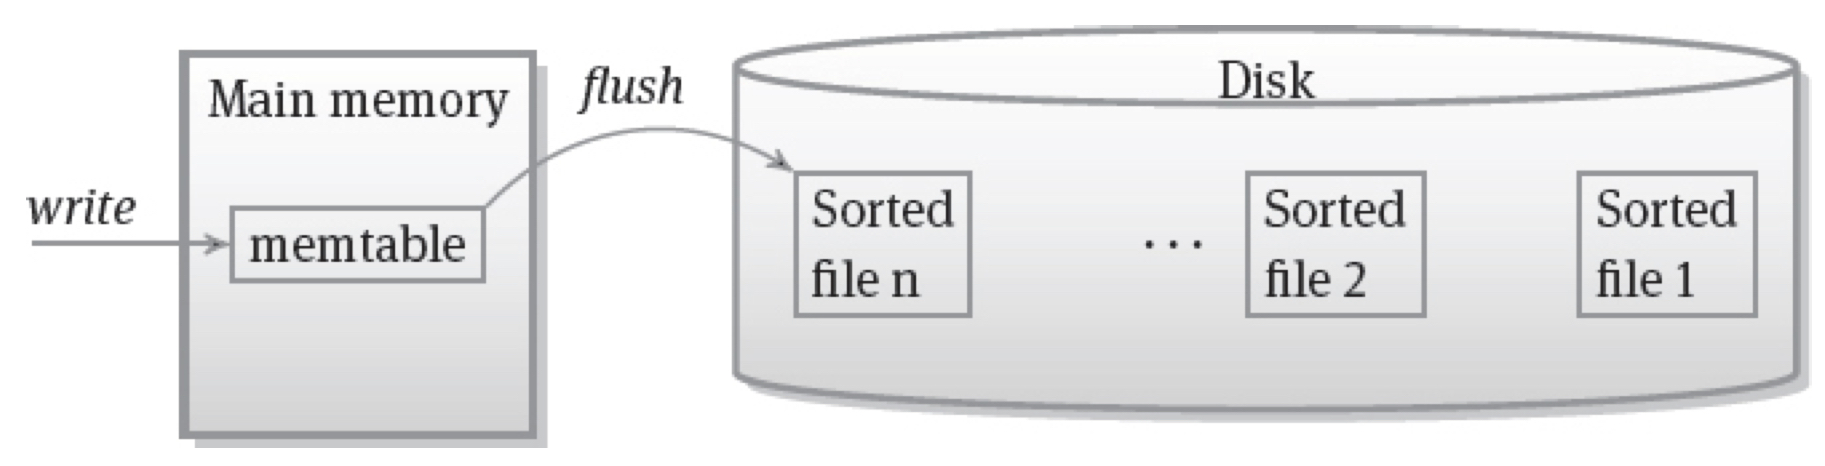
\includegraphics[width=0.70\linewidth]{images/AdvancedDataManagment/extensible_record_store/writing.jpeg}
    \caption{Writing to memory tables and data files}
\end{figure}

\subsubsection{Reading to memory tables and data files}
There are two types of read requests:
\begin{itemize}
    \item \textit{Get} also called \textbf{point query}. It accesses a particular row (identified by its row key).
    \item \textit{Scan} also called \textbf{range query}. It iterates over a contiguous range of rows depending on some condition on the row key.
\end{itemize}
\begin{figure}[!h]
    \centering
    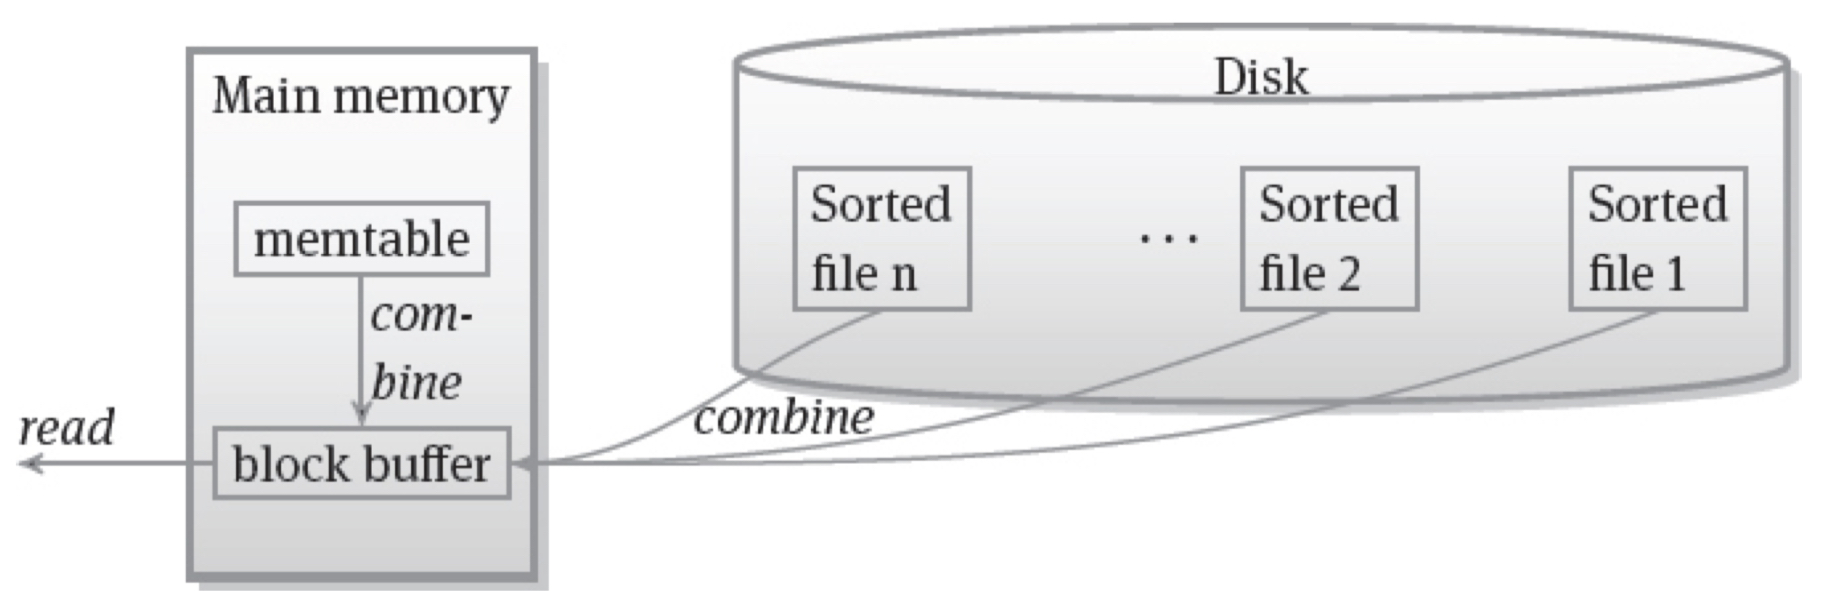
\includegraphics[width=0.70\linewidth]{images/AdvancedDataManagment/extensible_record_store/reading.jpeg}
    \caption{Reading to memory tables and data files}
\end{figure}


\newpage
\subsubsection{Consideration of both Reading and Writing operations}
More specifically, \textit{writing to} and \textit{reading from} an extensible record store comprises the following steps:
\begin{itemize}
    \item \textbf{Memtable:} 
    \begin{itemize}
        \item The most recent writes are collected in a main memory table of fixed size
        \item Usually there is one memtable per column family
        \item A record in the memtable is identified by its key (row key, column family, column qualifier and timestamp in milliseconds)
        \item Timestamp can be chosen by the user
        \item If no particular timestamp is specified in the put request, the current system time is used by default
    \end{itemize}
    \item \textbf{Tombstones:} 
    \begin{itemize}
        \item Deletions are treated by writing a new record for a key
        \item This record has no value assigned to it; instead a \textit{delete marker} (called \textbf{tombstone}) is attached to the record
        \item The tombstone masks all previous versions which will then be \textit{invisible to the user}
        \item A tombstone can for example \textbf{mark as deleted} either a \textit{single version of a column} or an \textit{entire column family}
    \end{itemize}
    \item \textbf{Sorted data files:} 
    \begin{itemize}
        \item Once the memtable is filled, it is written to disk (\textbf{flushed}) and an entirely new memtable is started. With this action its records are sorted by key
        \item The flushed sorted data files on disk are \textbf{immutable}
        \item The \textbf{advantage of immutable data files} is that \textit{buffer management} is a lot \textit{easier}: no dirty pages
    \end{itemize}
    \item \textbf{Combine upon read:} 
    \begin{itemize}
        \item The \textbf{downside} of immutable data files is that they \textbf{complicate the read process}
        \item Retrieving all the relevant data that match a user query requires combining records from several on-disk data files and the memtable
    \end{itemize}
\end{itemize}


Once the row keys to be accessed are identified, the result can be restricted to a subset of the columns inside each row. In some extensible record stores a set of versions of a cell can also be accessed. Usually, a \textit{range of timestamps} can also be specified in a per-query basis;

Combining records from various on-disk data files and the memtable and identifying the most recent version of a column is \textit{not trivial}, there may be a clash of timestamps.
\begin{itemize}
    \item If the user specifies a key that already exists in a data file, a new record with the same key is appended to the memtable and later on flushed to a new data file
    \item When reading this key, several values for exactly the same key could be returned from different data files
    \item Desirable to determine a unique most recent value for each key
    \item \textbf{Unique sequence number} of the stored data files:
    \begin{itemize}
        \item The record for a key that is contained in the data file with the highest sequence number is the most recently written one
    \end{itemize}
    \item Additional difficulty comes since the extensible record store has to \textit{interpret} the \textbf{time-to-live (TTL)} values of records as well as \textbf{tombstones} when retrieving and combining data from multiple sorted data files
\end{itemize}
Some \textit{extra information} can be maintained for each data file to speed up the combine process; for example, the \textbf{range of row keys} in the file or the \textbf{minimum and maximum timestamp} can be stored as metadata of the file.


\subsection{File format}
Extensible records stores store the data in the on-disk data files in a certain format with the following properties:
\begin{itemize}
    \item \textbf{Data blocks:}
    \begin{itemize}
        \item An on-disk data file is composed of several data blocks
        \item In some extensible record stores, a different block size can be used in each column family and hence the block size can be specified by the user when creating the column family
        \item A block may also span multiple conventional memory pages (fixed size by the memory buffer and the OS)
        \item Memory management is even more flexible in extensible record stores
    \end{itemize}
    \item \textbf{Key-value pairs:}
    \begin{itemize}
        \item A data block may contain one or more key-value pairs
        \item Each key-value pair contains the entire key
        \item This format hence is the foundation for the flexibility of extensible record stores because no fixed database schema is needed to interpret the data
        \item This flexibility however comes at the price of \textit{repetitious occurrences} of portions of keys
        \begin{itemize}
            \item Row consists of several columns
            \item Row key is contained in every record for each of these columns
            \item Column families and column qualifiers are usually parts of keys in several different records
        \end{itemize}
        \item The \textbf{key} is followed by the \textbf{type} information, it determines if the record is a put (\textit{upsert}) in which case a new value is appended or if it is a \textit{deletion}
    \end{itemize}
    \item \textbf{Index:}
    \begin{itemize}
        \item Data files usually contain records for several keys and may become quite large
        \item \textit{Reading} records in a data file sequentially is a very inefficient method when searching for a single record for a given key in such a large data file
        \item To \textbf{speed up} the process an index structure is maintained at the end of each file
        \item The first row key on each block is inserted in the index
        \item When searching for a given key in a data file, first of all the entire index of the data file is loaded into main memory
        \item As not all row keys are maintained in the index, the index has to return either the entry for the exact search, or the index entry for the largest row key preceding the search key
        \item In the later case the exact search key is not found in the index and we hence cannot be sure whether a record for the search key is contained in the data file or not
    \end{itemize}
    \item \textbf{Trailer:} as the last component of a data file, a trailer contains management information, like where the index starts
    
    \begin{figure}[!hbp]
    \centering
    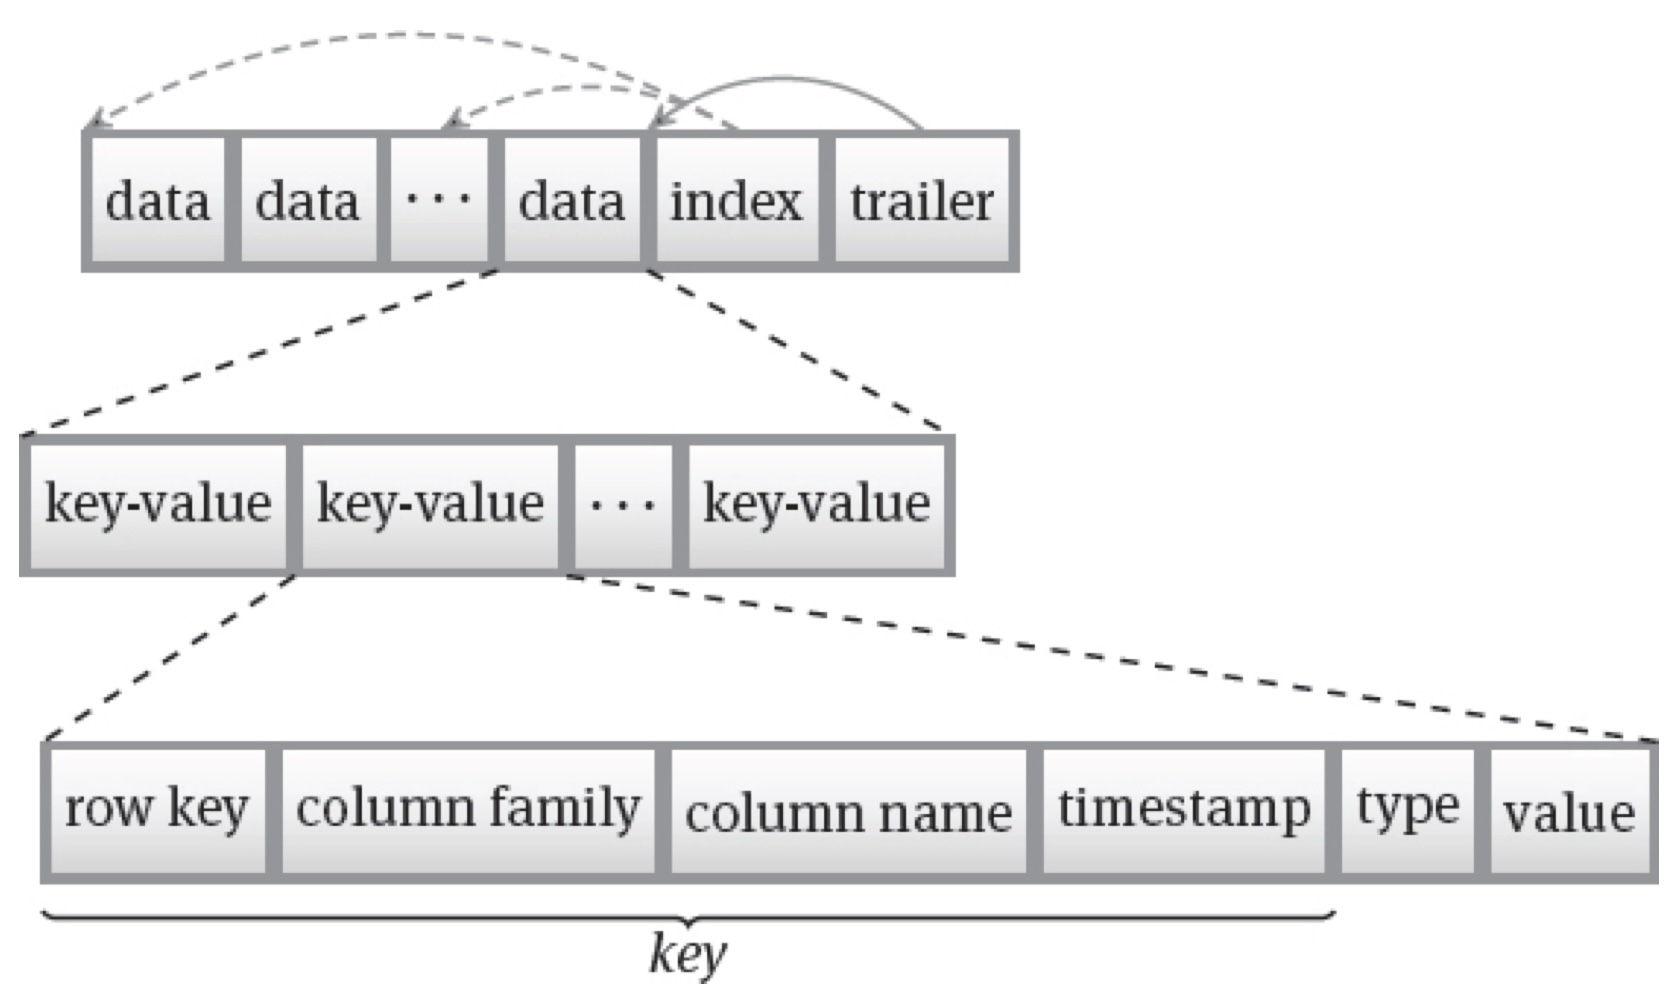
\includegraphics[width=0.50\linewidth]{images/AdvancedDataManagment/extensible_record_store/file_format.jpeg}
    \caption{File format of data files}
\end{figure}
    
    \item \textbf{Multi-level index:}
    \begin{itemize}
        \item Even though indexing is done at the block level and hence not all row keys are maintained in the index, the single index at the end of each data file might become quite large
        \item Might slow down the read process because the entire index has to be loaded into main memory before accessing any key-value pairs
        \item A multilevel index \textbf{splits the single index} into several \textit{sub-indexes}:
        \begin{itemize}
            \item One sub-index (\textit{leaf index}) is stored at the end of each block
            \item Only a small super-index (\textit{root index})  pointing to the sub-indexes is stored at the end of the data file
        \end{itemize}
    \end{itemize}
\end{itemize}

\section{Redo Logging}
\begin{itemize}
    \item The memtable is kept in volatile memory until it is eventually flushed to disk
    \item Data are only durable when stored in the on-disk data files and hence data that are contained in the memtable are vulnerable to failures of the database server
    \item \textbf{For example:} a crash of the server may wipe out the entire memory, or write errors may occur when flushing the memtable to disk
    \item When restarting the server the data in the memtable have to be recovered
\end{itemize}
\textbf{Recovery} is achieved with the help of an on-disk log file that keeps track of all records that are appended to the memtable but have not yet been flushed to the disk. This means that all data have be \textit{written twice} (log file and memtable).
\begin{itemize}
    \item Inside the log file, each record received a log sequence number (\textbf{LSN}) that maintains the \textit{chronological order} of write operations
    \item Since the data is stored to the \textit{on-disk log file} before appending them to the memtable, this process is called \textbf{write-ahead logging}
\end{itemize}

\begin{figure}[!hbp]
    \centering
    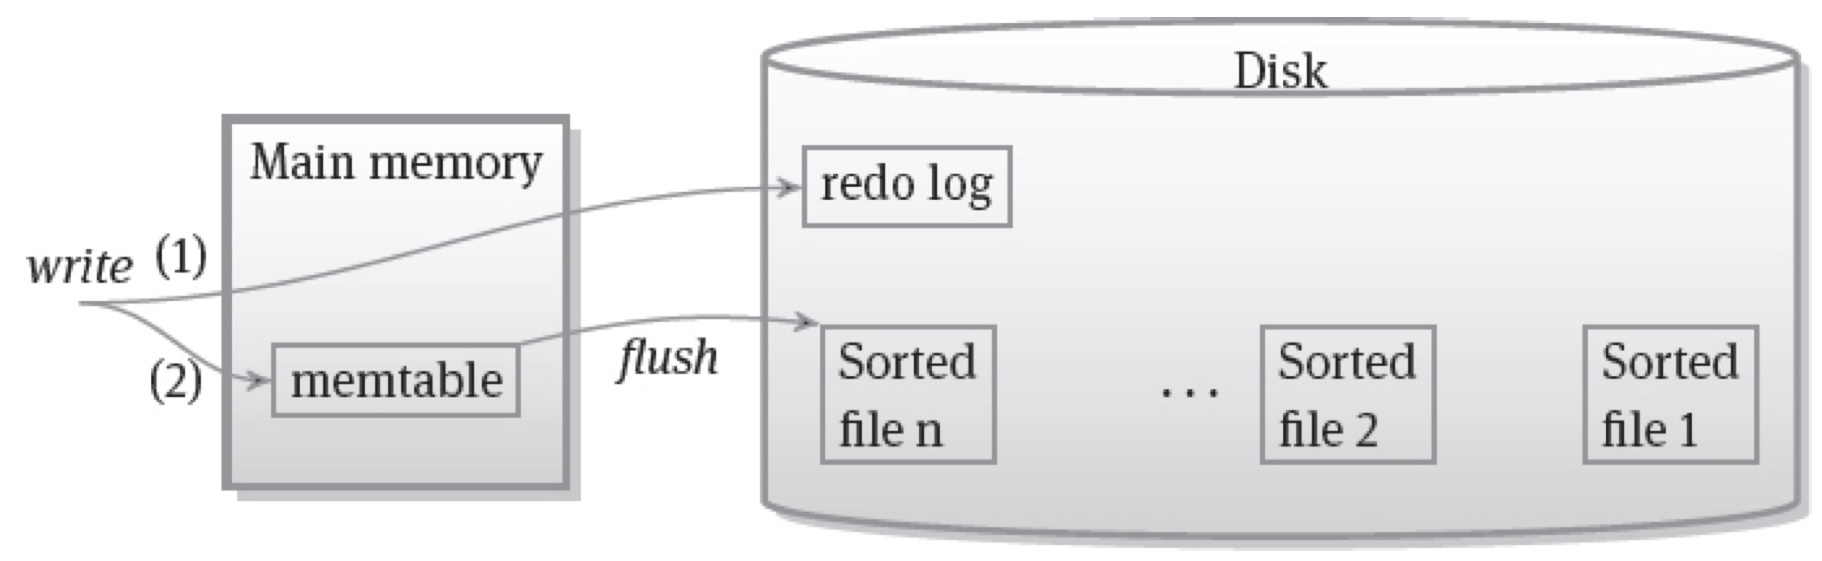
\includegraphics[width=0.70\linewidth]{images/AdvancedDataManagment/extensible_record_store/write_ahead_logging.jpeg}
    \caption{Write ahead log on disk}
\end{figure}

One peculiarity of extensible record stores is that they assume \textbf{redo-logging} to be \textit{sufficient}:
\begin{itemize}
    \item  When restarting the database server after a failure the memtable is reconstructed from the log file by re-executing all the operations in the log as ordered by their LSNs.
    \item Remarking the fact that extensible record stores do not support transactions and long-lived transaction
\end{itemize}
Although the logging mechanism \textbf{adds an additional overhead} to the write process, it in fact \textbf{improves overall write performance}: while appending a record to the log file in \textit{chronological order} is fast, sorting the records by key is \textit{slower} and can be deferred until flushing the memtable.

Last but not least, writes to the same key can be melted (fuso) and only the most recent record has to be flushed to disk. In particular, \textbf{no record} for a key must be \textbf{written} to disk at all if an \textit{upsert} for the key is \textit{masked} by a \textbf{tombstone} for the key in the memtable.


\subsection{Compaction}
After some time, several flushes of memtables will have occurred and hence there will be quite a lot of data files stored on disk, in which probably contain some outdated records:
\begin{itemize}
    \item Records whose time-to-live value has passed
    \item Records for which more recent versions exist
    \item Records for which the maximum numbe r of stored versions is exceeded
    \item Records which are masked by a tombstone
\end{itemize}
All this kind of data \textit{slow down read} processes because they have to be loaded and compared with other records in the combine process of data retrieval. This is why a process called \textbf{compaction} was devised to remove any unwanted records and merge a set of data files into a new one.

\begin{figure}[!hbp]
    \centering
    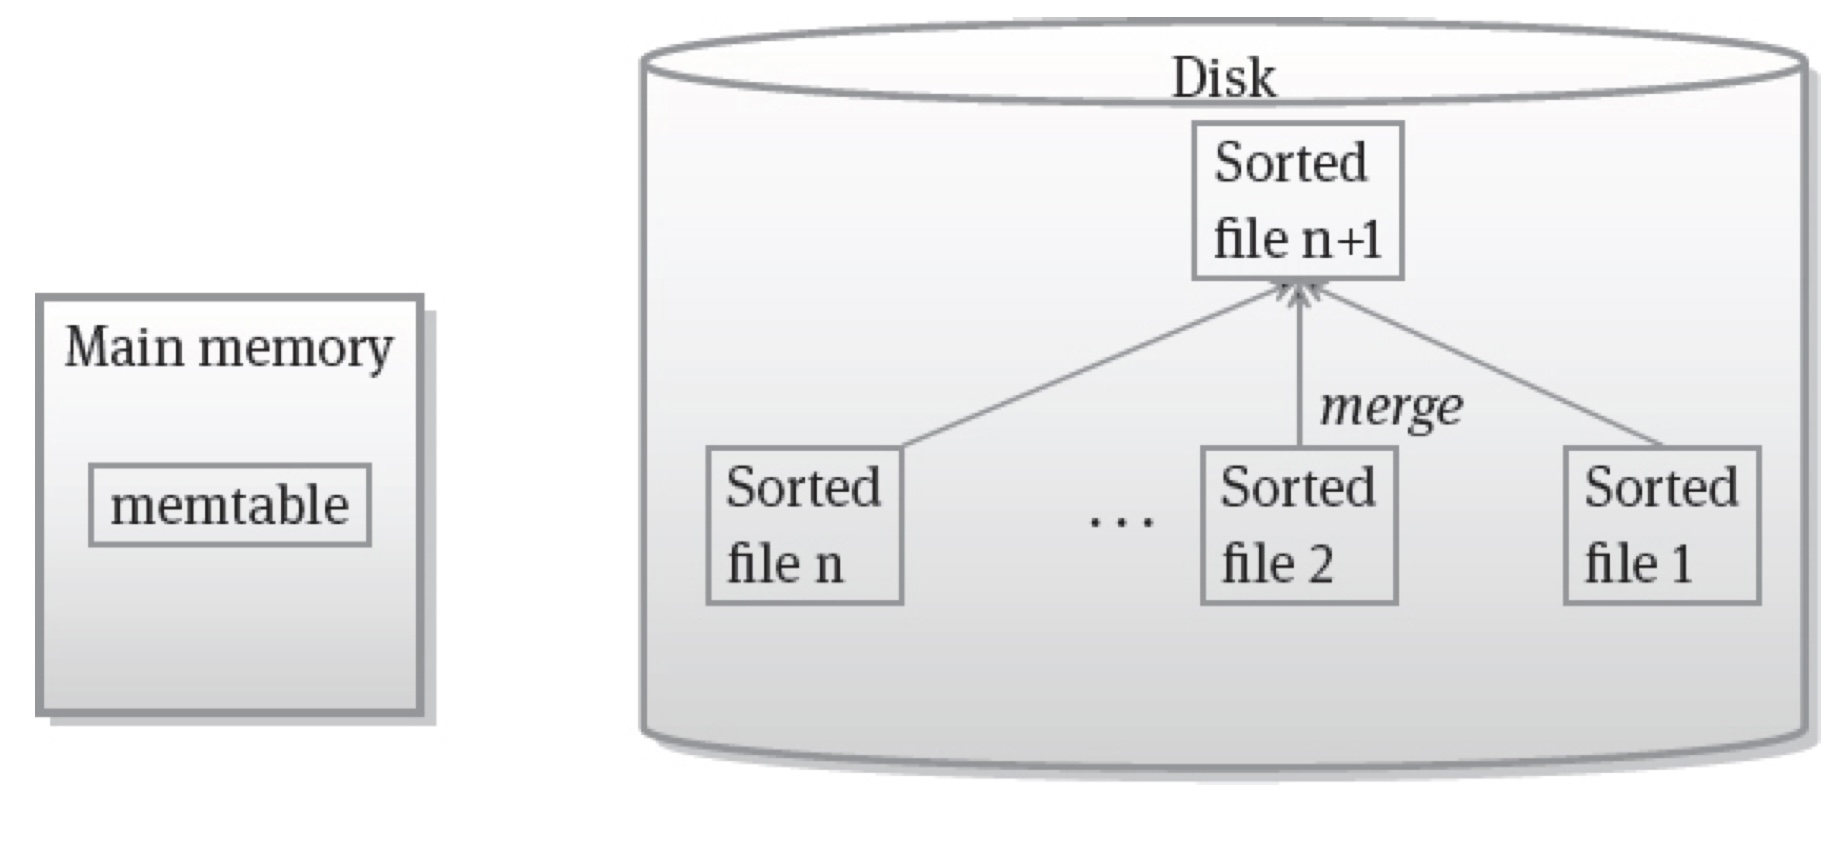
\includegraphics[width=0.70\linewidth]{images/AdvancedDataManagment/extensible_record_store/comapct.jpeg}
    \caption{Compaction on disk}
\end{figure}

In this example image a set of data file is chosen for compaction, so their records are merged and the result is written to a new larger data file.
\begin{itemize}
    \item \textbf{Minor compaction:} merges only a small subset of all data files
    \item \textbf{Major compaction:} merges all data files into a single new one
\end{itemize}
Several things have to be considered during compaction:
\begin{itemize}
    \item Records have to be sorted by key thus the index have to be reconstructed
    \item Time-to-live values have to be interpreted to ignore invalid records
    \item If a tombstone is in a data file, all file marked by it and those written before the arrival of the tombstone can be ignored
    \begin{itemize}
        \item Records that are masked by the tombstone but have been \textit{written after} the insertion of the tombstone are \textit{handled differently}: they are merged into the new data file but they still be masked by the tombstone if it is a \textit{minor compaction}
        \item \textbf{Tombstones} themselves can only be \textit{deleted} during \textbf{major compaction}
        \item So only after a major compaction more recent records for a key will be visible because they would previously be masked by the tombstone
    \end{itemize}
    \item In some extensible record stores, \textit{versioning settings} are also enforced during compaction: only a specified amount of versions for each key is kept at the maximum
    \item \textbf{Changing column family} settings can be done during \textit{major compaction}
\end{itemize}
Compaction is demanding with respect to disk space. While the compaction process is running twice the disk space as occupied by the smaller data files. However they will be discarded after compaction effectively releasing the disk space.

Several \textbf{heuristics} can be applied when choosing data files \textbf{for minor compaction:}
\begin{itemize}
    \item \textbf{Oldest files first:} chronologically ordered data file in which the oldest files with the lowest sequence number are chosen for compaction
    \item \textbf{Small files first:} to obtain a \textit{homogeneous set} of data files, several similar sized smaller files are merged into one larger file
    \item \textbf{Compaction threshold:} the user can configure a minimum number of files for which a compaction is run
\end{itemize}
Note that with these heuristics, the same record may be chosen for minor compaction several times and the records unnecessarily often migrates from smaller files into larger files.

Furthermore, the \textbf{size of the resulting compacted} files \textit{cannot be controlled}. To avoid this, \textbf{leveled compaction} has been developed:
\begin{itemize}
    \item Data files are organized into levels
    \item Data files in lower levels are smaller than data files in higher levels
    \item A \textbf{flush} always moves the memtable to a data file in the \textit{lowest level L0}
    \item \textit{Subsequent compaction} steps move a record only from one level to the next, so amount of merges for each record is bounded by the number of levels
\end{itemize}

\begin{figure}[!hbp]
    \centering
    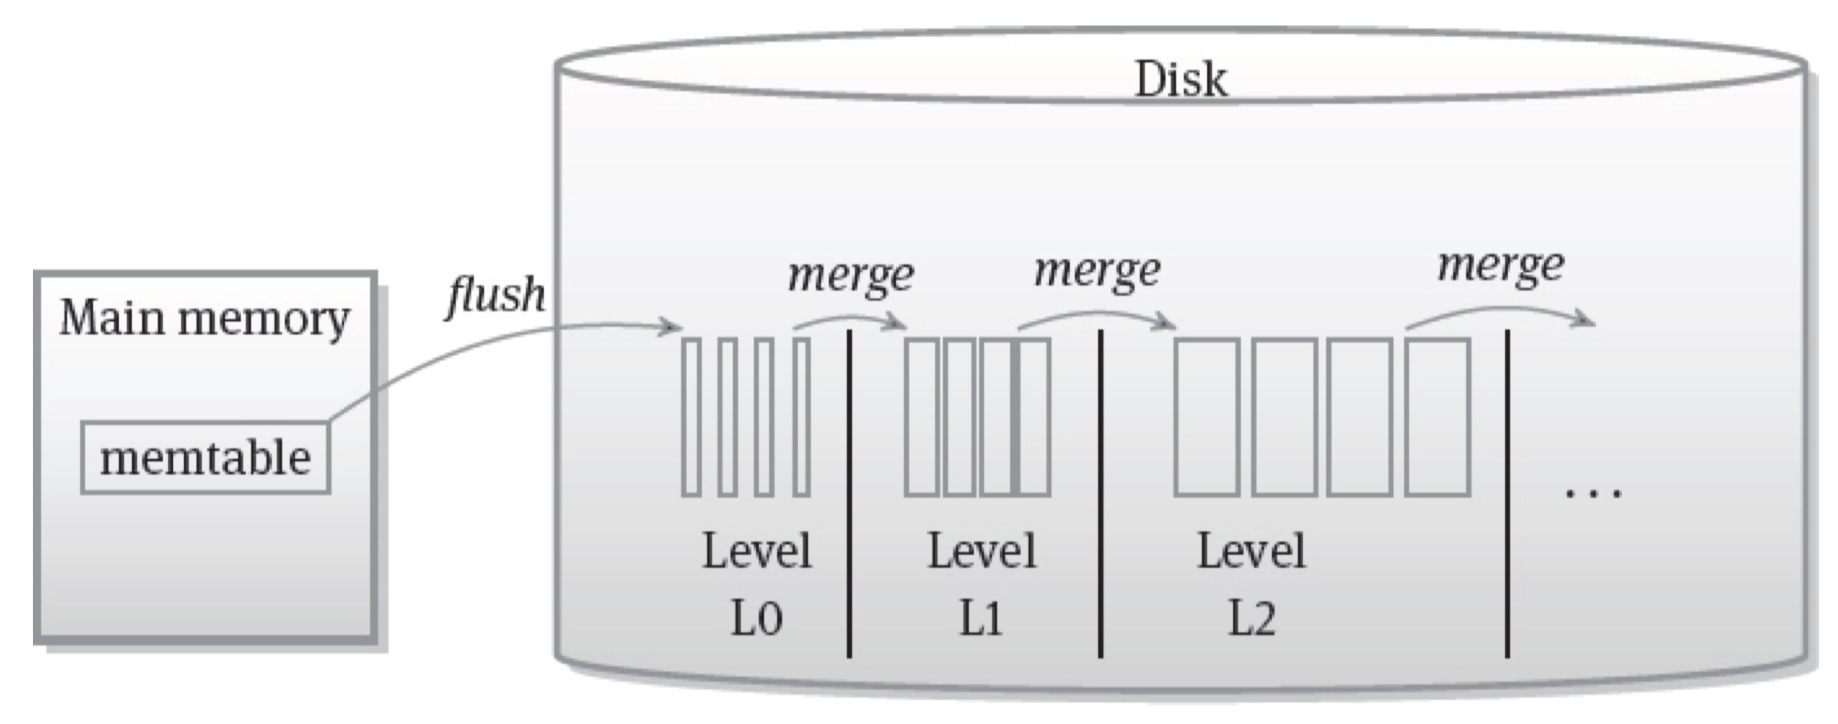
\includegraphics[width=0.70\linewidth]{images/AdvancedDataManagment/extensible_record_store/leveled_compaction.jpeg}
    \caption{Level compaction}
\end{figure}

\subsection{Bloom filters}
A Bloom filter is a probabilistic method to determine set membership for a given value.
\begin{tcolorbox}
For a given value \(c\) and a set \(S\) of values, the \textbf{Bloom filter} is a \textbf{small bit vector} with which we can decide whether \(c\) is \textit{included} in \(S\) without actually searching for \(c\) in \(S\). Of course it comes with a small probability of error.
\end{tcolorbox}

\begin{itemize}
    \item \textbf{True positive:} Bloom filter \textbf{correctly} reports a \textbf{match} and confirms that \(c\) is an element of \(S\). So \(c \in S\) holds
    \item \textbf{False positive:} Bloom filter \textbf{wrongly} reports a \textbf{match}, so it though that\(c \in S\) but actually \(c \notin S\)
    \item \textbf{True negative:} Bloom filter \textbf{correctly} reports a \textbf{miss}, so \(c \notin S\) holds;
    \item \textbf{False negative:} Bloom filter \textbf{erroneously} reports a \textbf{miss}, so it though that\(c \notin S\) but actually \(c \in S\)
\end{itemize}
The only kind of error that could arises are \textbf{False positives}:
\begin{itemize}
    \item When the Bloom filter reports a match we cannot be sure if this is true
    \item We have to actually search for \(c\) in \(S\) to verify whether \(c \in S\) holds
    \item Or whether the Bloom filter wrongly believed \(c\) to be an element of \(S\) although in fact \(c \notin S\) holds
\end{itemize}

For extensible record stores, Bloom filters \textit{can be maintained} for all the row keys in a data file with the following positive effect:
When searching for a given query key in the file, first the Bloom filter is accessed with the query key. If the Bloom filter reports a
\begin{itemize}
    \item \textbf{Miss:} \textit{true negative}, so we do not have to access any data
    \item \textbf{Match:} we have to load the index and search it for the query key to check whether the match was a \textit{true positive} or a \textit{false positive} (which means the record is not found in the data file)
\end{itemize}
Moreover for
\begin{itemize}
    \item \textbf{Small data files:} a single Bloom filter can be appended at the end of the data file
    \item \textbf{Large data file} with lots of keys: a single Bloom filter will be too large. So this will result in performance delays when searching for a row key in the data file.
\end{itemize}
Bloom filter can be broken into pieces, a small Bloom filter “chunk” is maintained for the keys in each block; the Bloom filter chunk is then queried for the existence of a key before actually accessing data in the corresponding block.

\begin{tcolorbox}
A \textbf{Bloom filter} is a bit vector of a chosen length \(m\)
with every position initialized to 0. The bit vector is accompanied by
\(k\) different hash functions \((h_1,...,h_k)\) where each hash function is
assumed to map an arbitrary value \(c\) randomly to a number between
1 and \(m\) – that is, \((h_i(c) \in {1,...,m})\).
\end{tcolorbox}

For each number \(d\) between 1 and \(m\), the probability that an input value \(c\) is mapped to \(d\) should be equal to \(\frac{1}{m}\) this ca be written as \textit{Prob}\((h_i(c) = d) = \frac{1}{m}\)

The case that \textbf{two different input values} \(c\) and \(c'\) are mapped to the same value, so \(h_i(c) = h_i(c')\) we will have a so called \textbf{collision}. Collisions are the reason why false positives can occur with Bloom filter.
\newpage
\begin{figure}[!h]
    \centering
    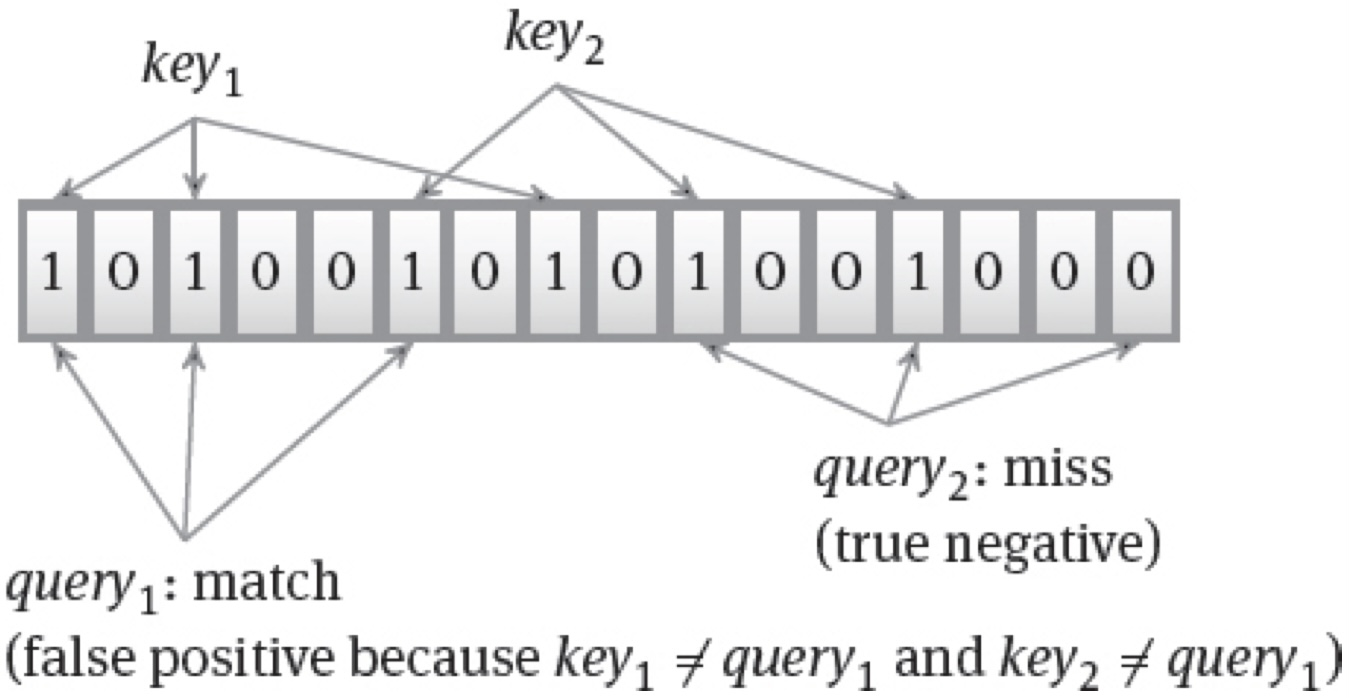
\includegraphics[width=0.50\linewidth]{images/AdvancedDataManagment/extensible_record_store/bloom_filter.jpeg}
    \caption{Bloom filter}
\end{figure}

The rate of false positive is approxiamted as:
\begin{tcolorbox}
\[\biggl(1 - \biggl(1 - \frac{1}{m}\biggl)^{k \cdot n}\biggl)^k \approx (1 - e^{\frac{-k \cdot n}{m}})^k\]
\end{tcolorbox}
With \(k\) as the number of hash functions, \(m\) as the Bloom Filter length and \(n\) as the number of input keys.